\documentclass{article}
\usepackage{ctex}
\usepackage{makecell}
\usepackage{graphicx}
\usepackage{geometry}
\usepackage{multirow}
\usepackage{multicol}
\usepackage{fancyhdr}
\usepackage{longtable}
\usepackage{color}
\usepackage{float}
\usepackage{listings}
\usepackage{xcolor}
\usepackage{hyperref}
\usepackage{footnote}
\usepackage{paralist}
\usepackage{amsmath}

\let\itemize\compactitem
\let\enditemize\endcompactitem
\let\enumerate\compactenum
\let\endenumerate\endcompactenum
\let\description\compactdesc
\let\enddescription\endcompactdesc

\geometry{a4paper,left=25mm,right=20mm,top=25mm,bottom=25mm}

\title{数字图像处理实验二}
\author{09021227~金桥}
\date{\today}

\lstset{
    numbers=left,
    keywordstyle= \color{ blue!70},
    commentstyle= \color{red!50!green!50!blue!50},
    rulesepcolor= \color{ red!20!green!20!blue!20} ,
    % escapeinside=``,
    numberstyle=\tt,
    numbersep=0em,
    xleftmargin=2em,
    breaklines,
    aboveskip=1em,
    framexleftmargin=2em,
    frame=shadowbox,
    basicstyle=\tt,
    language=C++
}

\begin{document}

\maketitle

\section{实验目标}

\subsection{第一部分}
构建一个灰度值全是1的灰度图像,加入一定方差的高斯白噪声(要能看到明显的噪声),判断频谱图是否接近水平;
阅读论文,对Non-Local Means算法的中心思想进行理解和总结。
对Lena灰度图像加入高斯噪声,分别对其进行中值处理、均值处理、自适应中值处理、Non-Local Means处理并进行图像对比。

\subsection{第二部分}

对Lena灰度图像加入一定密度的椒盐噪声(要能看到明显的噪声),分别对其进行中值处理、均值处理、自适应中值处理、Non-Local Means处理并进行图像对比 (这个要结合课上的自适应中值滤波器思路,进行结合)

\section{过程与方法}

请注意,以下算法均为自主手动实现,\textbf{没有调用OpenCV的方法。}

\subsection{高斯白噪声生成}

高斯白噪声的生成采用了C++11自带的高斯随机生成器。仍然基于原有框架,对每个像素点叠加一个高斯分布随机数并保证结果位于0与255之间。
其中生成的随机数均值为0,标准差为20.
\subsection{椒盐噪声生成}

椒盐噪声的实现相对比较简单,使每个像素点有 $\frac{30}{256}$ 的概率变成 0 或者 255 即可.

\subsection{中值处理}

最开始的想法是遍历每个像素点,将周围范围内的像素点取出排序,然后取出中值。但是发现速度实在太慢。因此采用以下算法:

\begin{enumerate}
    \item 每行最开始生成一个直方图,内容为范围内的像素点。
    \item 处理时从左到右遍历直方图并求和,如果求和大于范围内的像素点数量的一半,则中值为对应值。
    \item 向右移动时从直方图中减去左侧的像素点,并将右侧的像素点添加至直方图中。
\end{enumerate}

思考了一下,原来的算法时间复杂度为 $O(n^2(m^2+m\log m))$, 换用这种算法则可以降低至 $O(n^2m)$. 因此速度会变快不少。
除此以外,原来的算法要分配空间并排序,这个操作的常数较大,也是原来算法慢的一个原因。

\subsection{均值处理}

采用跟上面的方法类似的逻辑:

\begin{enumerate}
    \item 每行最开始统计范围内像素点的和。
    \item 向右移动时从和中减去左侧的像素点之和,并将右侧的像素点之和添加和中。
\end{enumerate}

均值处理后的值就是当前和除以范围内像素点的数量。

\subsection{自适应中值处理}

自适应中值的实现实际上就是使得中值处理的窗口可以变化。设置有最大的窗口尺寸以及最小的窗口尺寸。

\begin{itemize}
    \item 如果当前窗口内灰度值的中值介于最大灰度值与最小灰度值之间:
    \begin{itemize}
        \item 当前像素也介于最大灰度值与最小灰度值之间,则保持不变。
        \item 否则,输出中值。
    \end{itemize}
    \item 否则,增大窗口大小重新进行,直到当前窗口已是最大。
\end{itemize}
\subsection{Non-Local Means}

Non-Local Means 处理后的值由以下公式给出:$$\text{NLMeans}(A)=\sum w(A, B)\times I(B)$$
其中:
$$w(A, B)=\frac{1}{\text{sum}}e^{-\frac{\text{MSE}(A, B)}{h^2}}$$
$$\text{sum}=\sum e^{-\frac{\text{MSE}(A, B)}{h^2}}$$
$$\text{MSE}(A, B)=\frac{1}{mn}\sum_{i=0}^{m-1}\sum_{j=0}^{n-1}(A(i, j)-B(i, j))^2$$
其中$A, B$ 分别是当前点的邻域块以及搜索窗口内其他点的邻域块,并且邻域块的大小为$m\times n$.

Non-Local Means的计算较多,因此生成图像的速度相对会比较慢一些。生成512大小的图像耗时大概是10秒左右。

\section{结果与分析}

\subsection{第一部分}

构建一个灰度值全是1的灰度图像并加入一定方差的高斯白噪声,并生成其傅里叶变换图像:

\begin{figure}[H]
    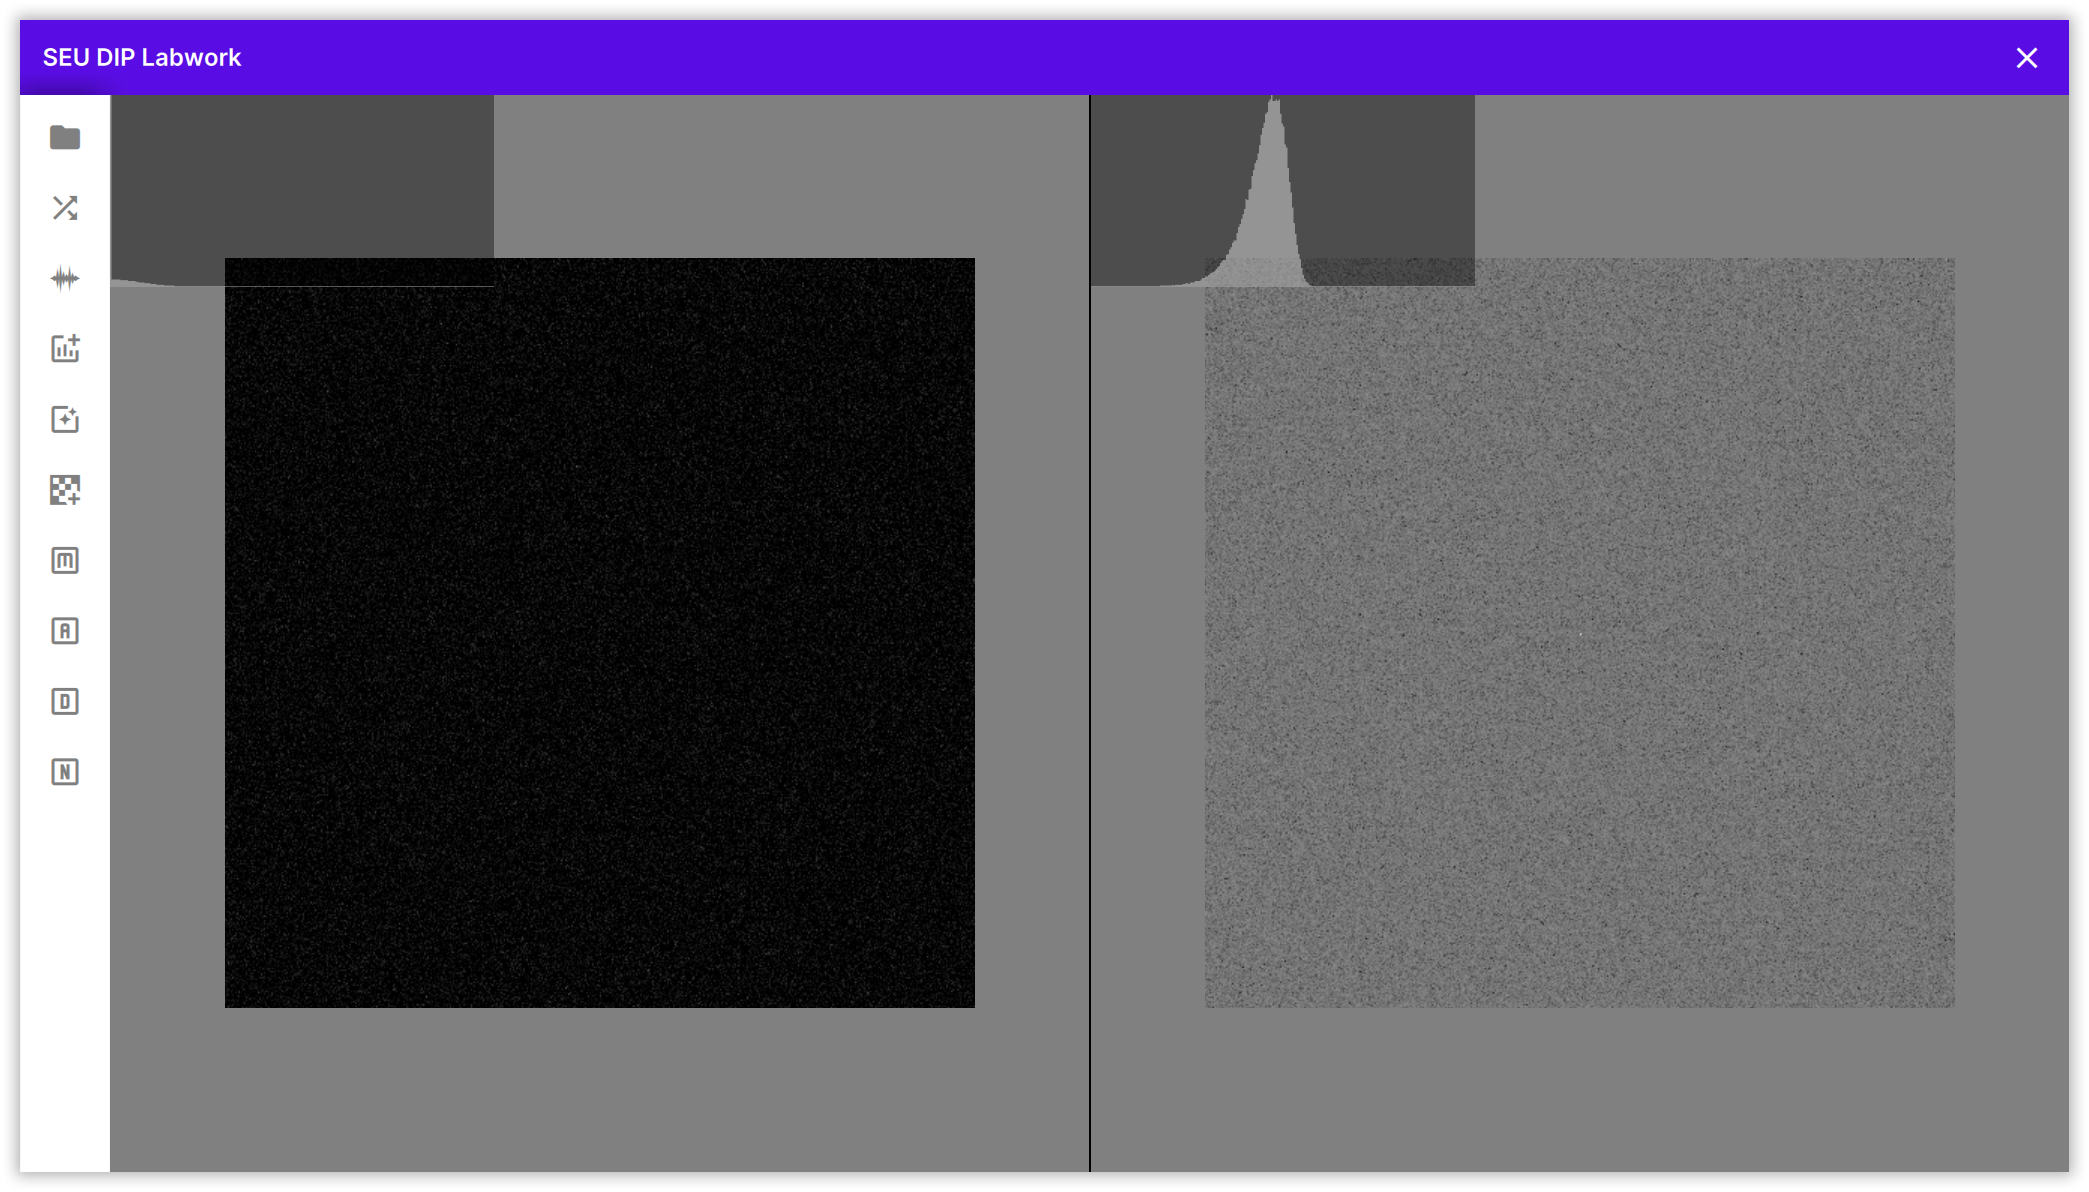
\includegraphics[width=\textwidth]{img/gaussian-fourier.png}
    \caption{左侧为添加高斯白噪声之后的图像,右侧是对应的傅里叶变换图像}
\end{figure}

可以看到,右侧傅里叶变换后的图像灰度比较均匀(直方图的峰值比较集中),频谱图接近水平。

我个人对于Non-Local Means算法的中心思想的理解与总结如下:它主要是利用了整幅图像进行降噪,以图像块为单位寻找相似区域并求平均,从而能够较好的去除均值为0的高斯白噪声。

接下来对Lena灰度图像加入高斯噪声并进行中值处理、均值处理、自适应中值处理以及Non-Local Means处理:

\begin{figure}[H]
    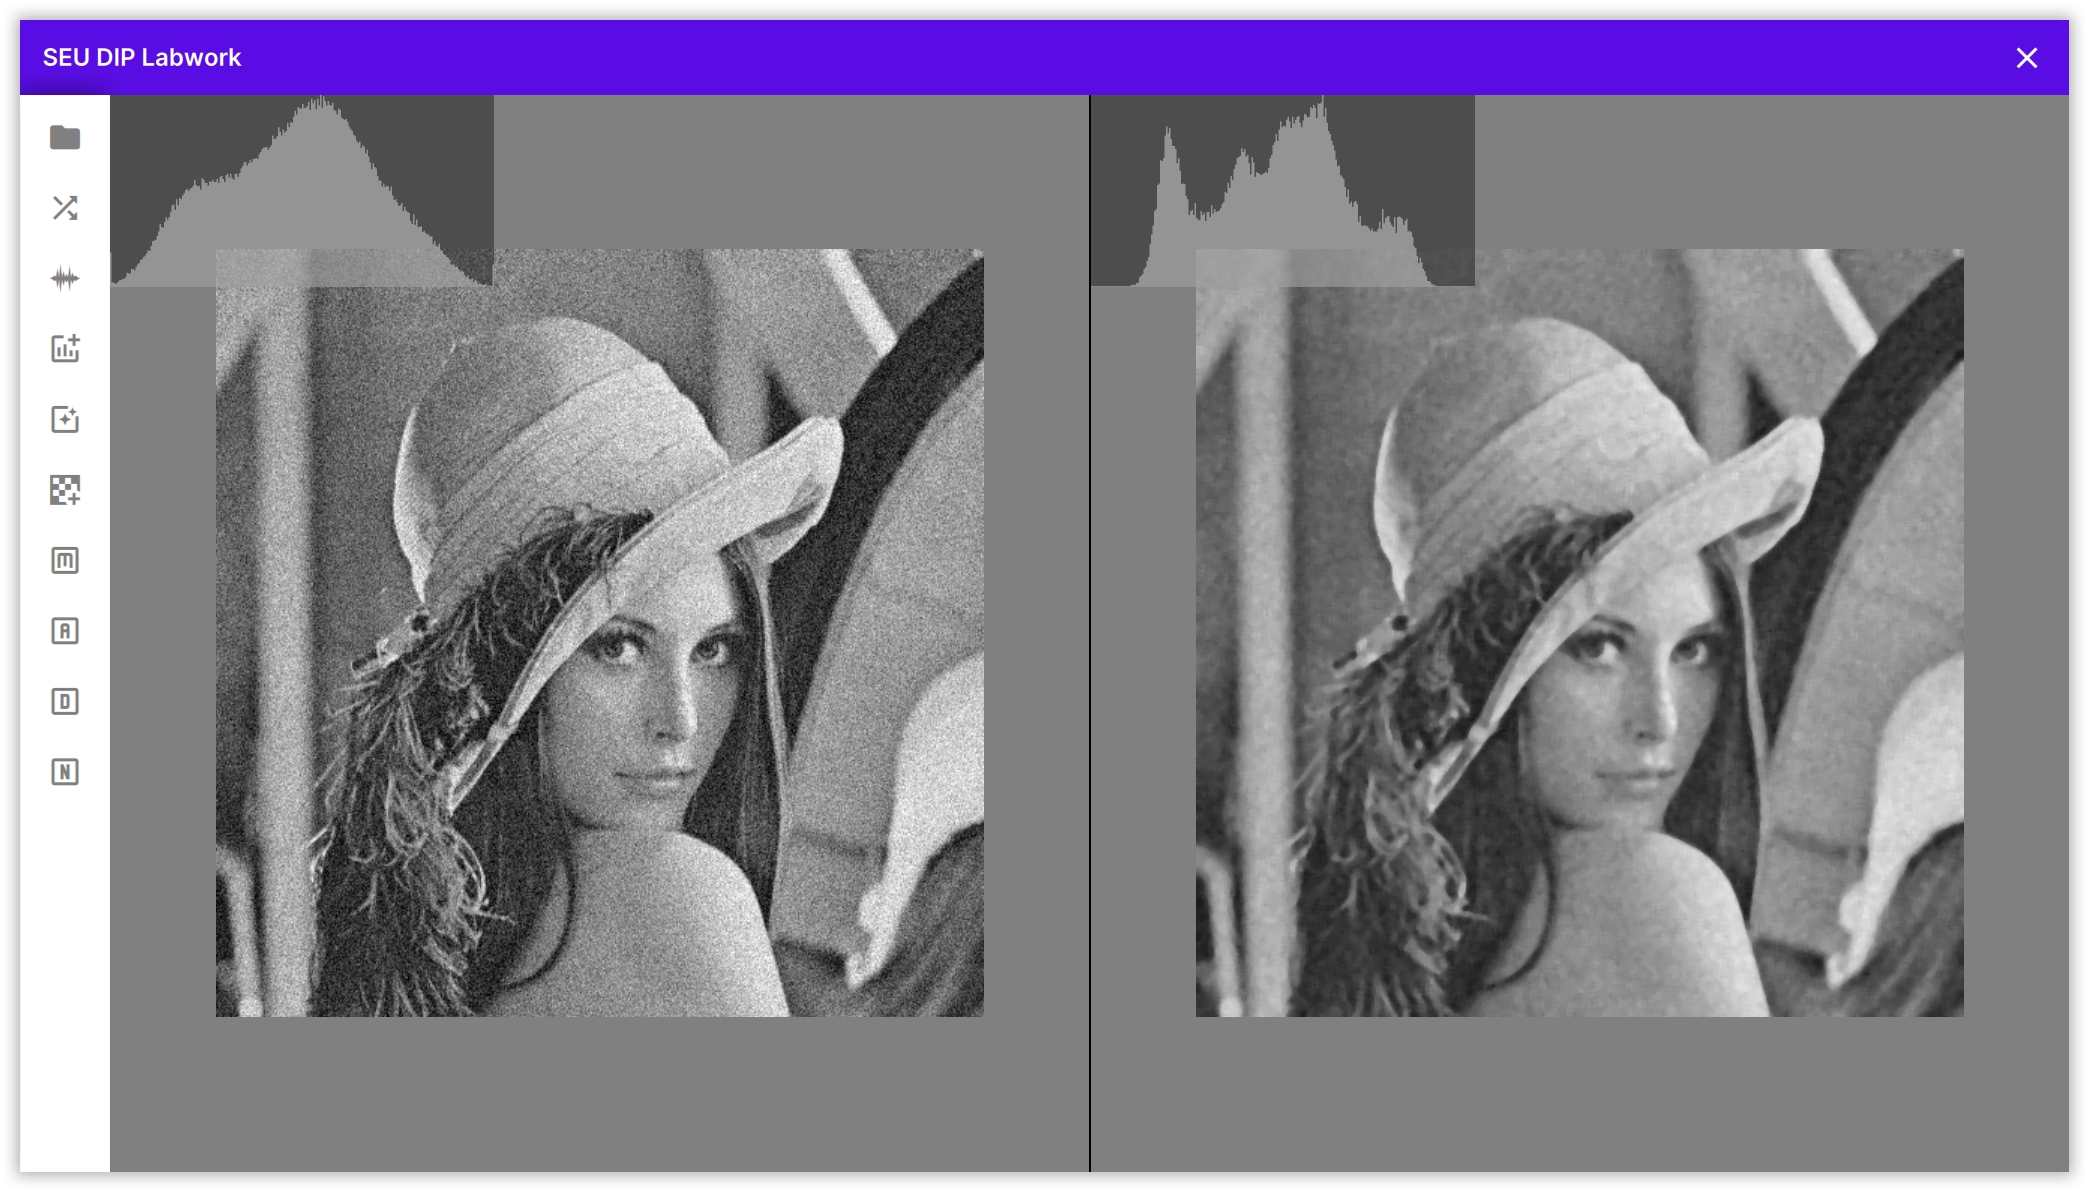
\includegraphics[width=\textwidth]{img/gaussian/lena-med.png}
    \caption{左侧为添加高斯白噪声之后的Lena图像,右侧是中值处理后的图像}
\end{figure}

\begin{figure}[H]
    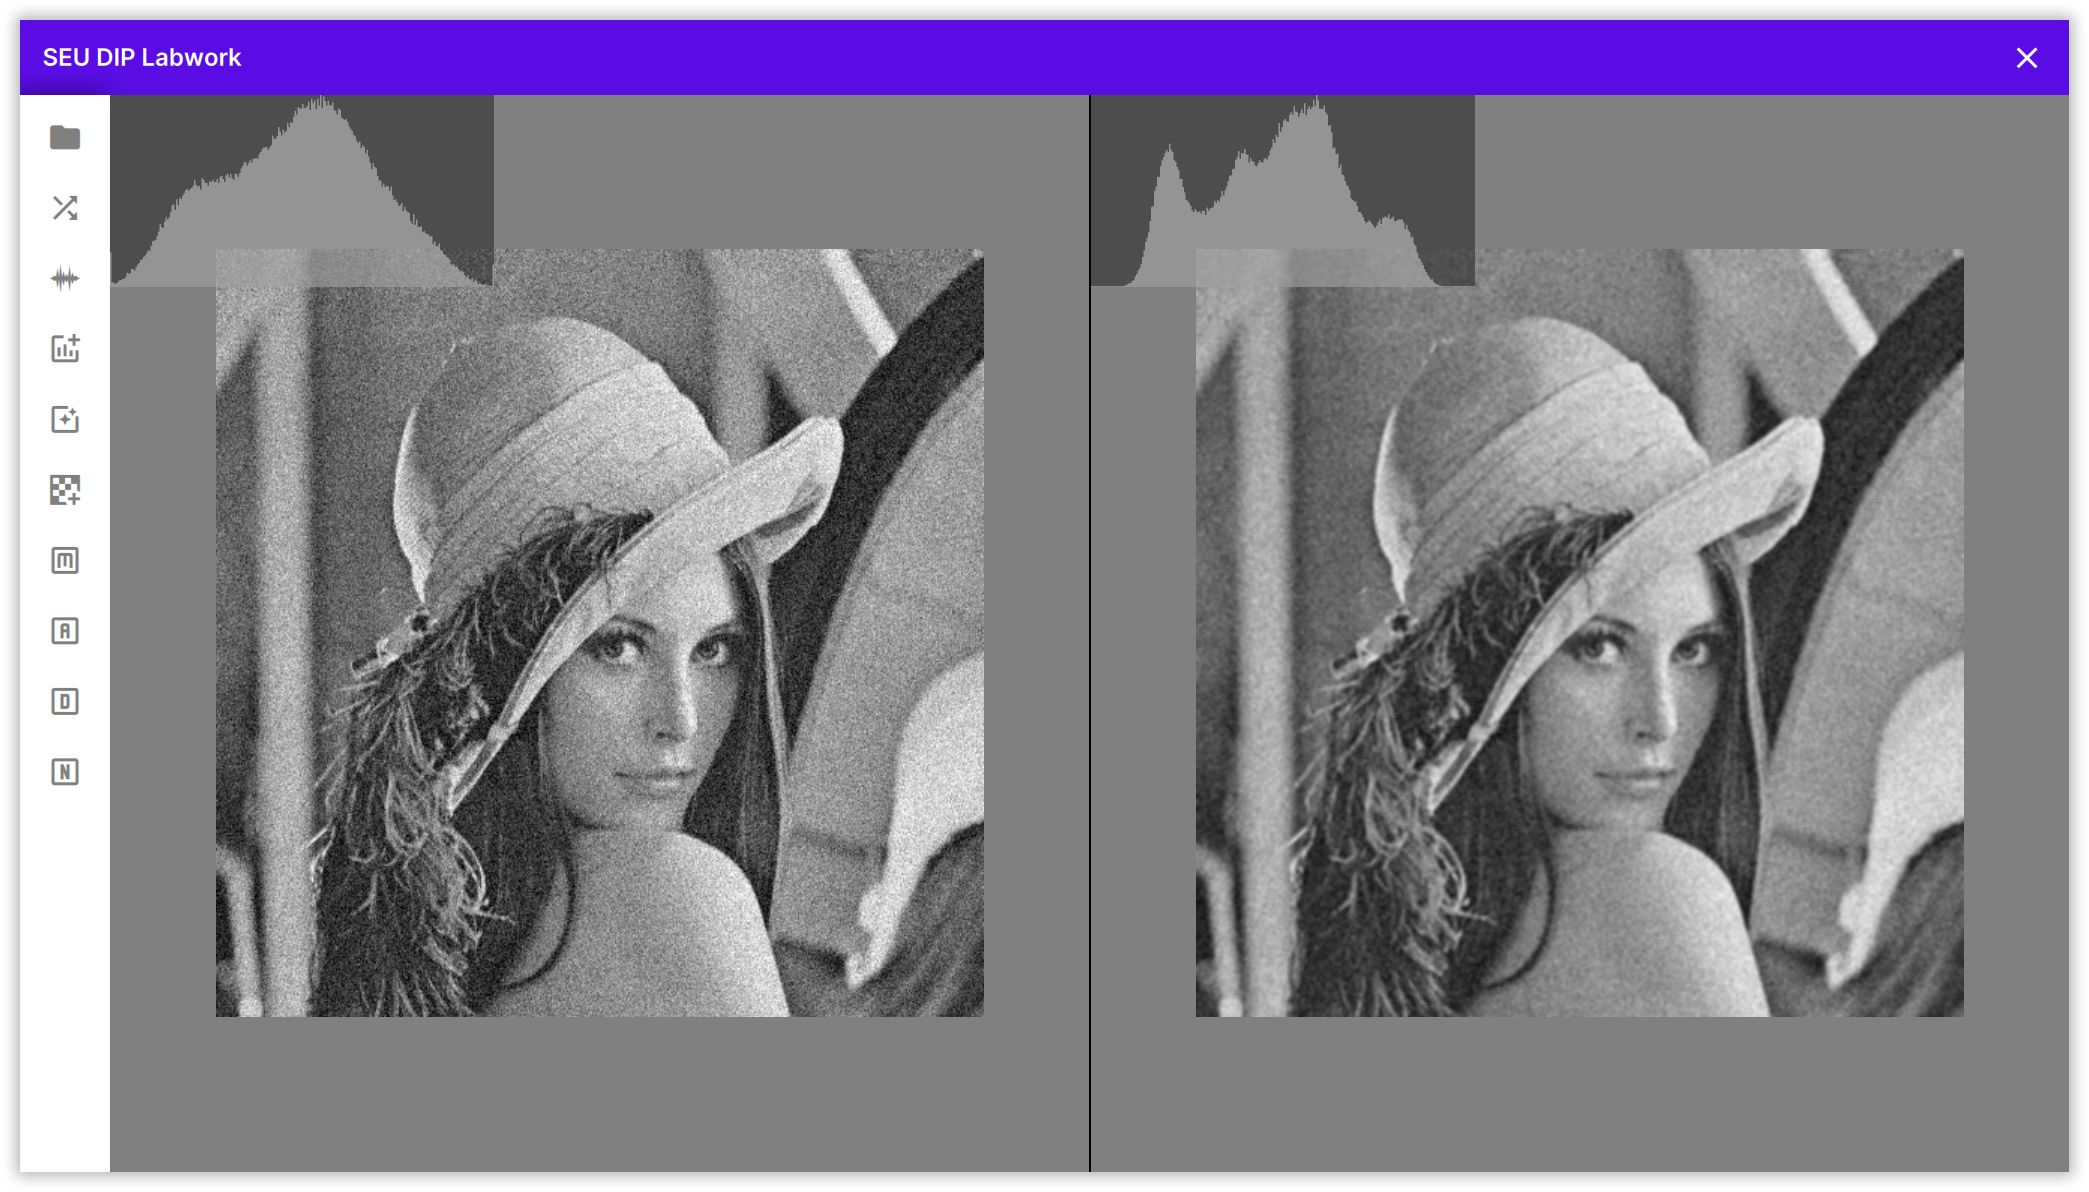
\includegraphics[width=\textwidth]{img/gaussian/lena-avg.png}
    \caption{左侧为添加高斯白噪声之后的Lena图像,右侧是均值处理后的图像}
\end{figure}

\begin{figure}[H]
    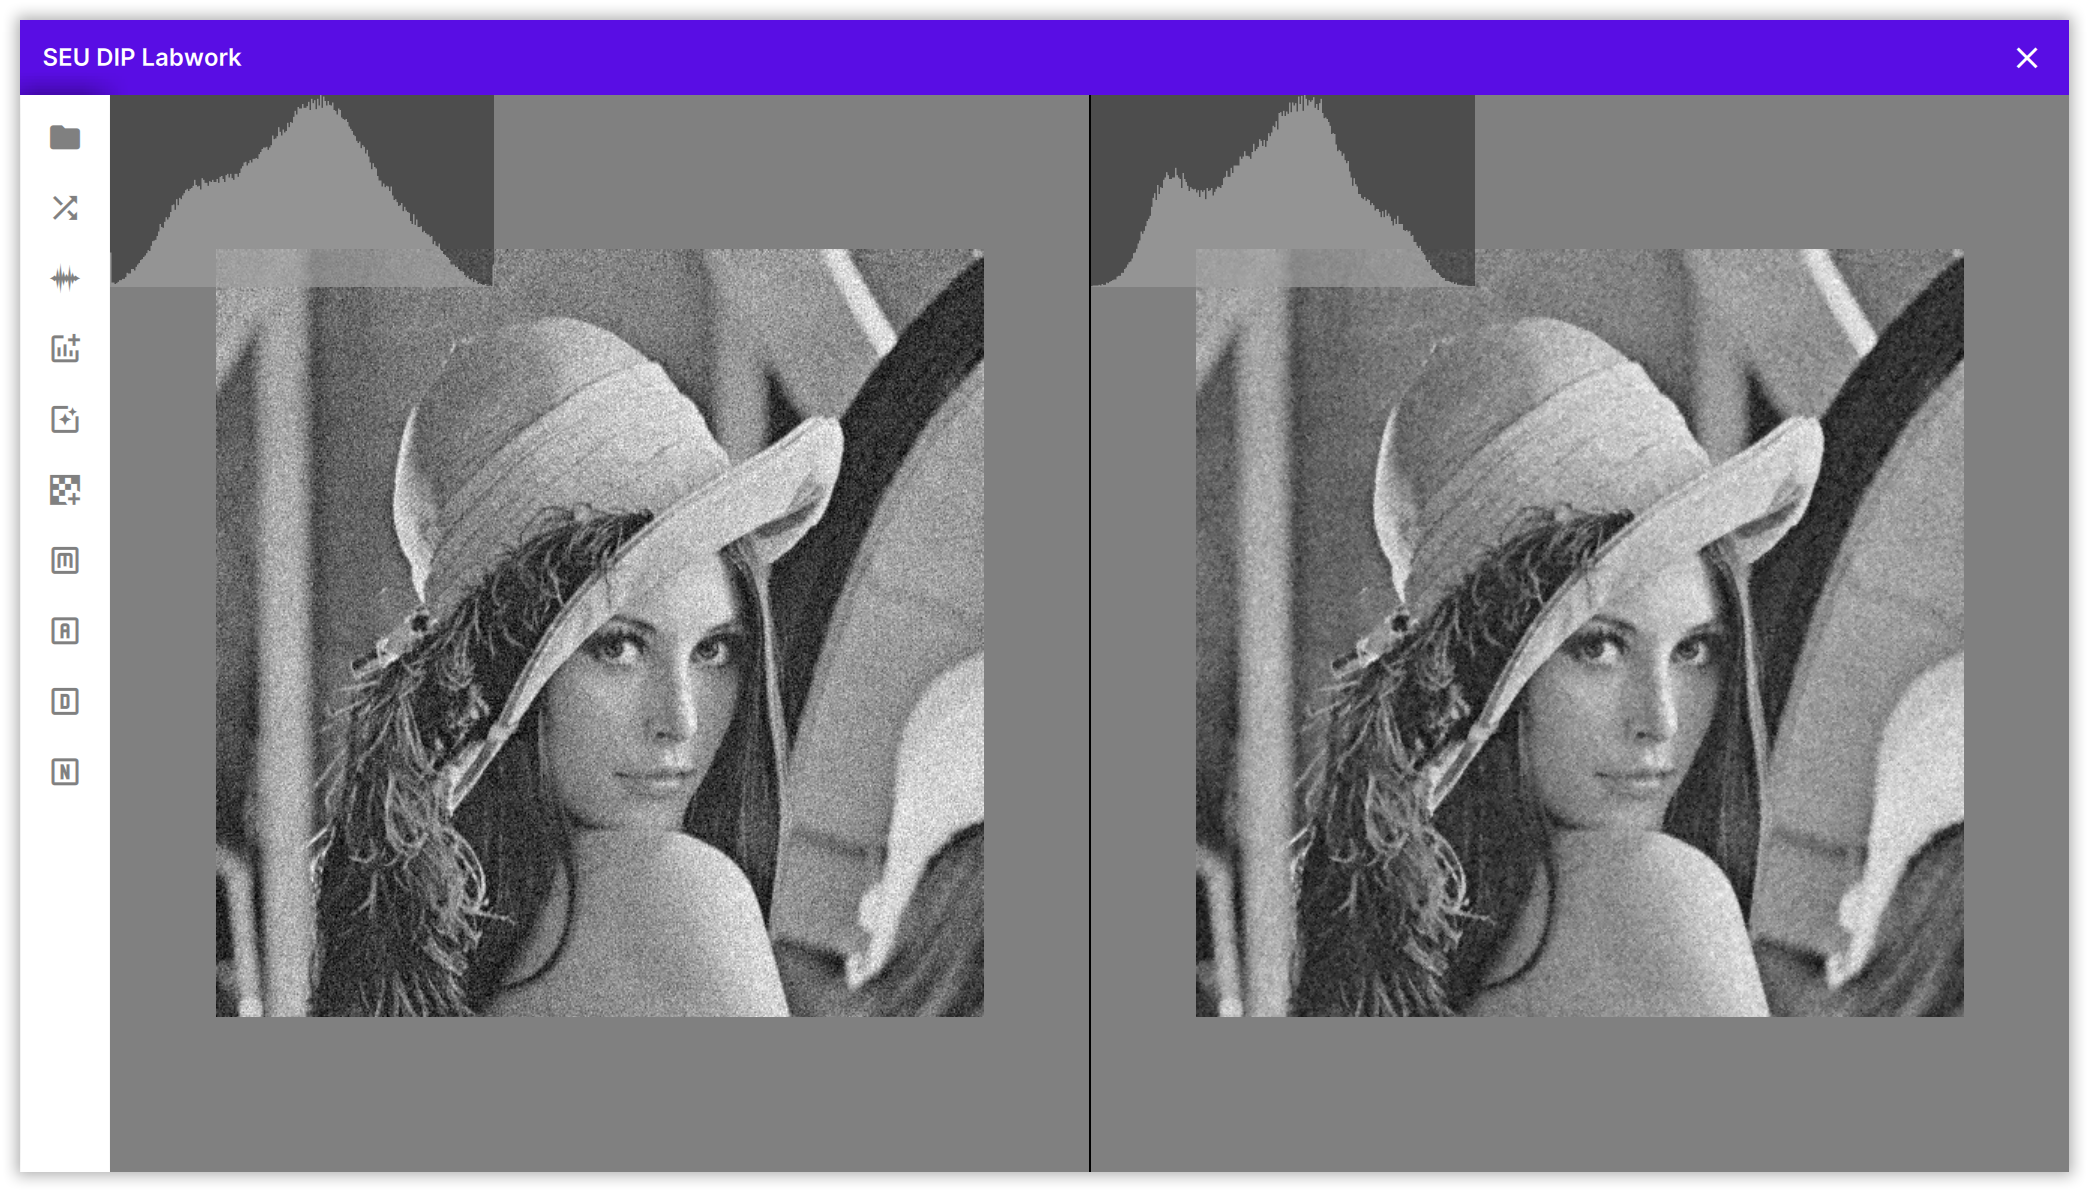
\includegraphics[width=\textwidth]{img/gaussian/lena-adaptive.png}
    \caption{左侧为添加高斯白噪声之后的Lena图像,右侧是自适应中值处理后的图像}
\end{figure}

\begin{figure}[H]
    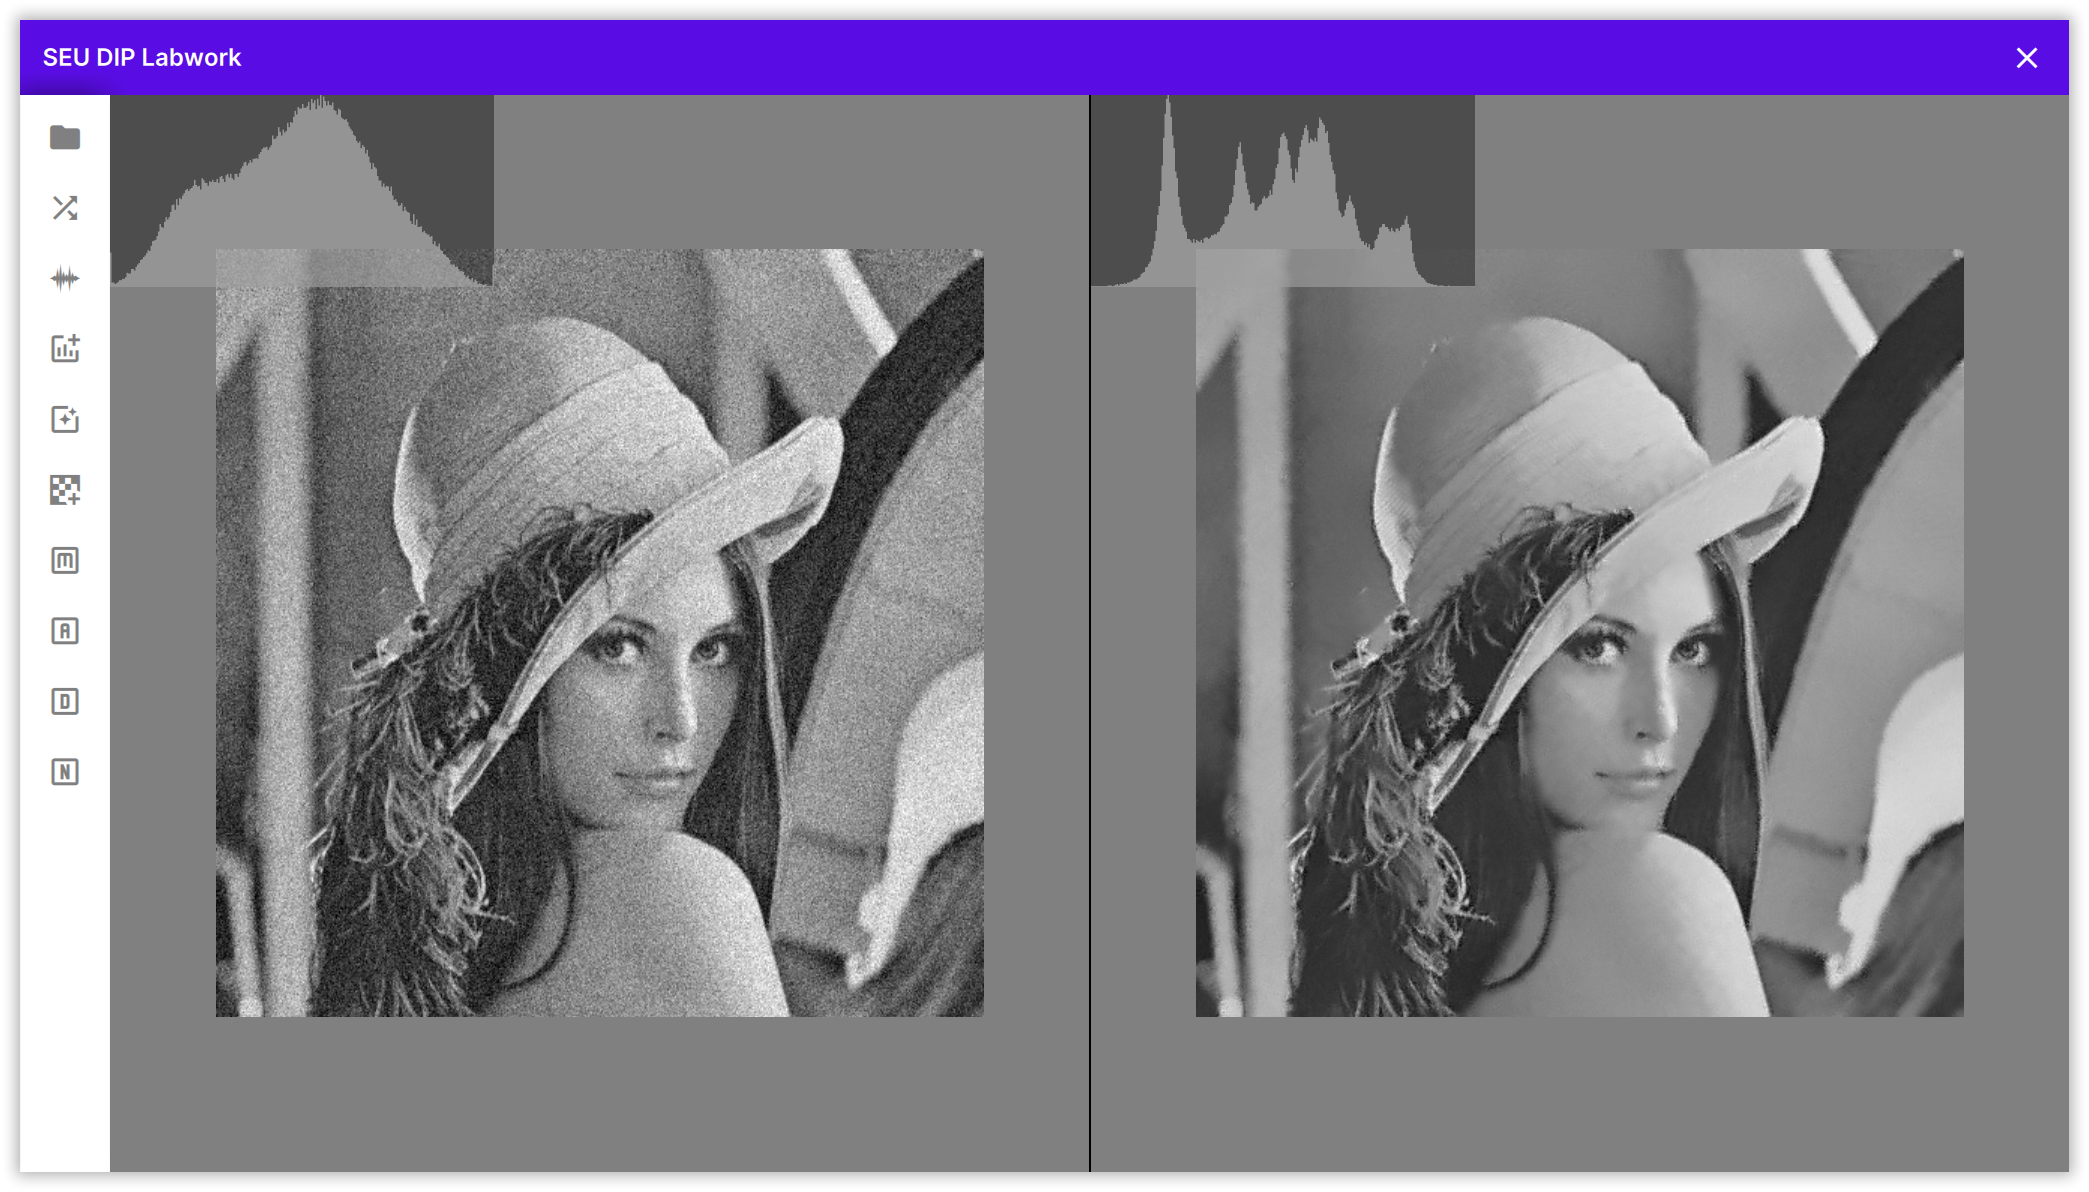
\includegraphics[width=\textwidth]{img/gaussian/lena-nonlocal.png}
    \caption{左侧为添加高斯白噪声之后的Lena图像,右侧是Non-Local Means处理后的图像}
\end{figure}

可以看到,中值处理、均值处理以及自适应中值处理对于高斯白噪声的降噪效果并不是很理想,而Non-Local Means方法可以有效的去除高斯白噪声。

\subsection{第二部分}

对Lena图像加入椒盐噪声并进行中值、均值、自适应中值处理以及Non-Local Means处理:

\begin{figure}[H]
    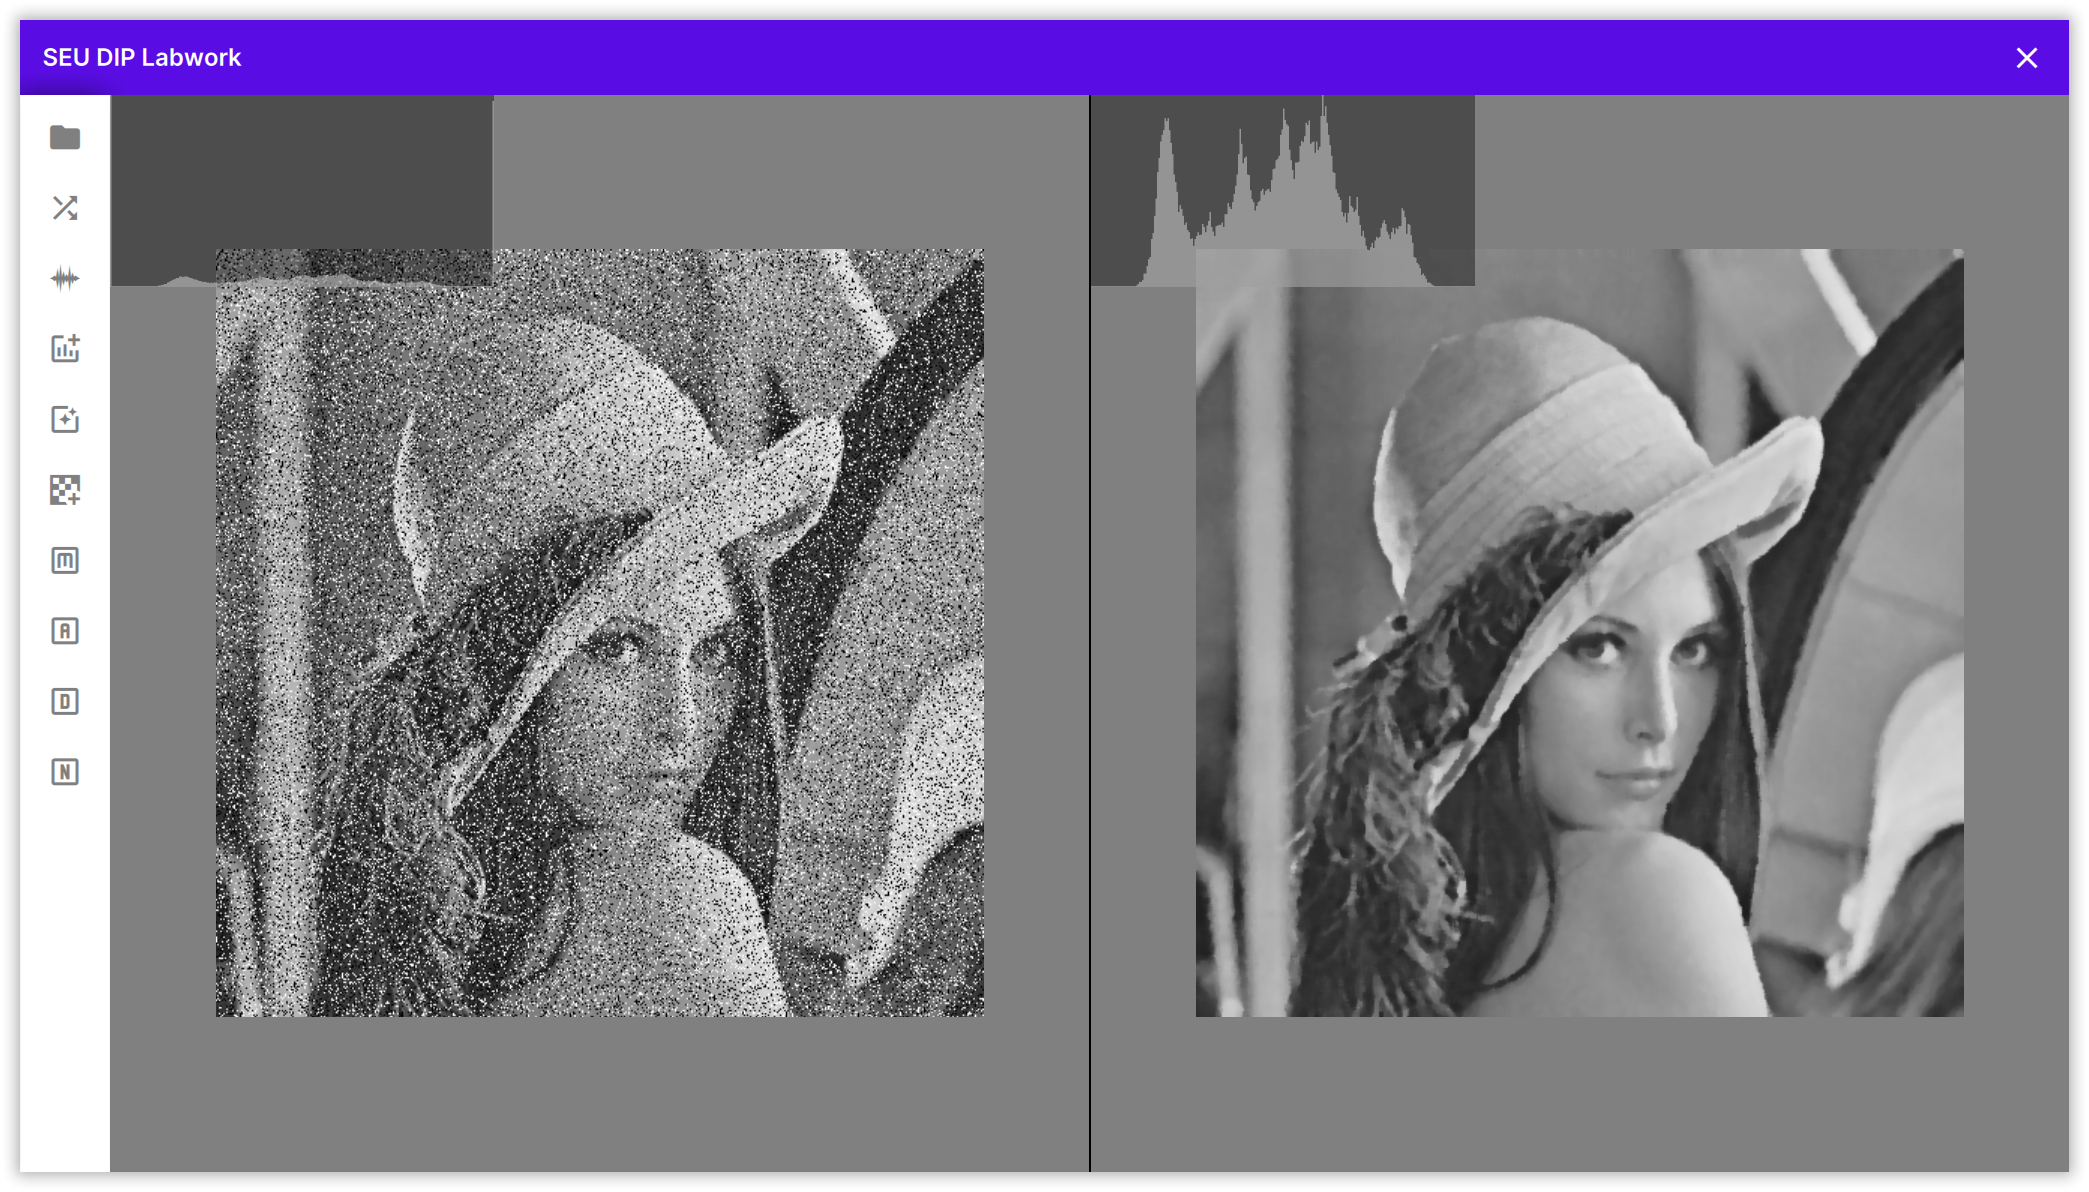
\includegraphics[width=\textwidth]{img/saltpepper/lena-med.png}
    \caption{左侧为添加椒盐噪声之后的Lena图像,右侧是中值处理后的图像}
\end{figure}

\begin{figure}[H]
    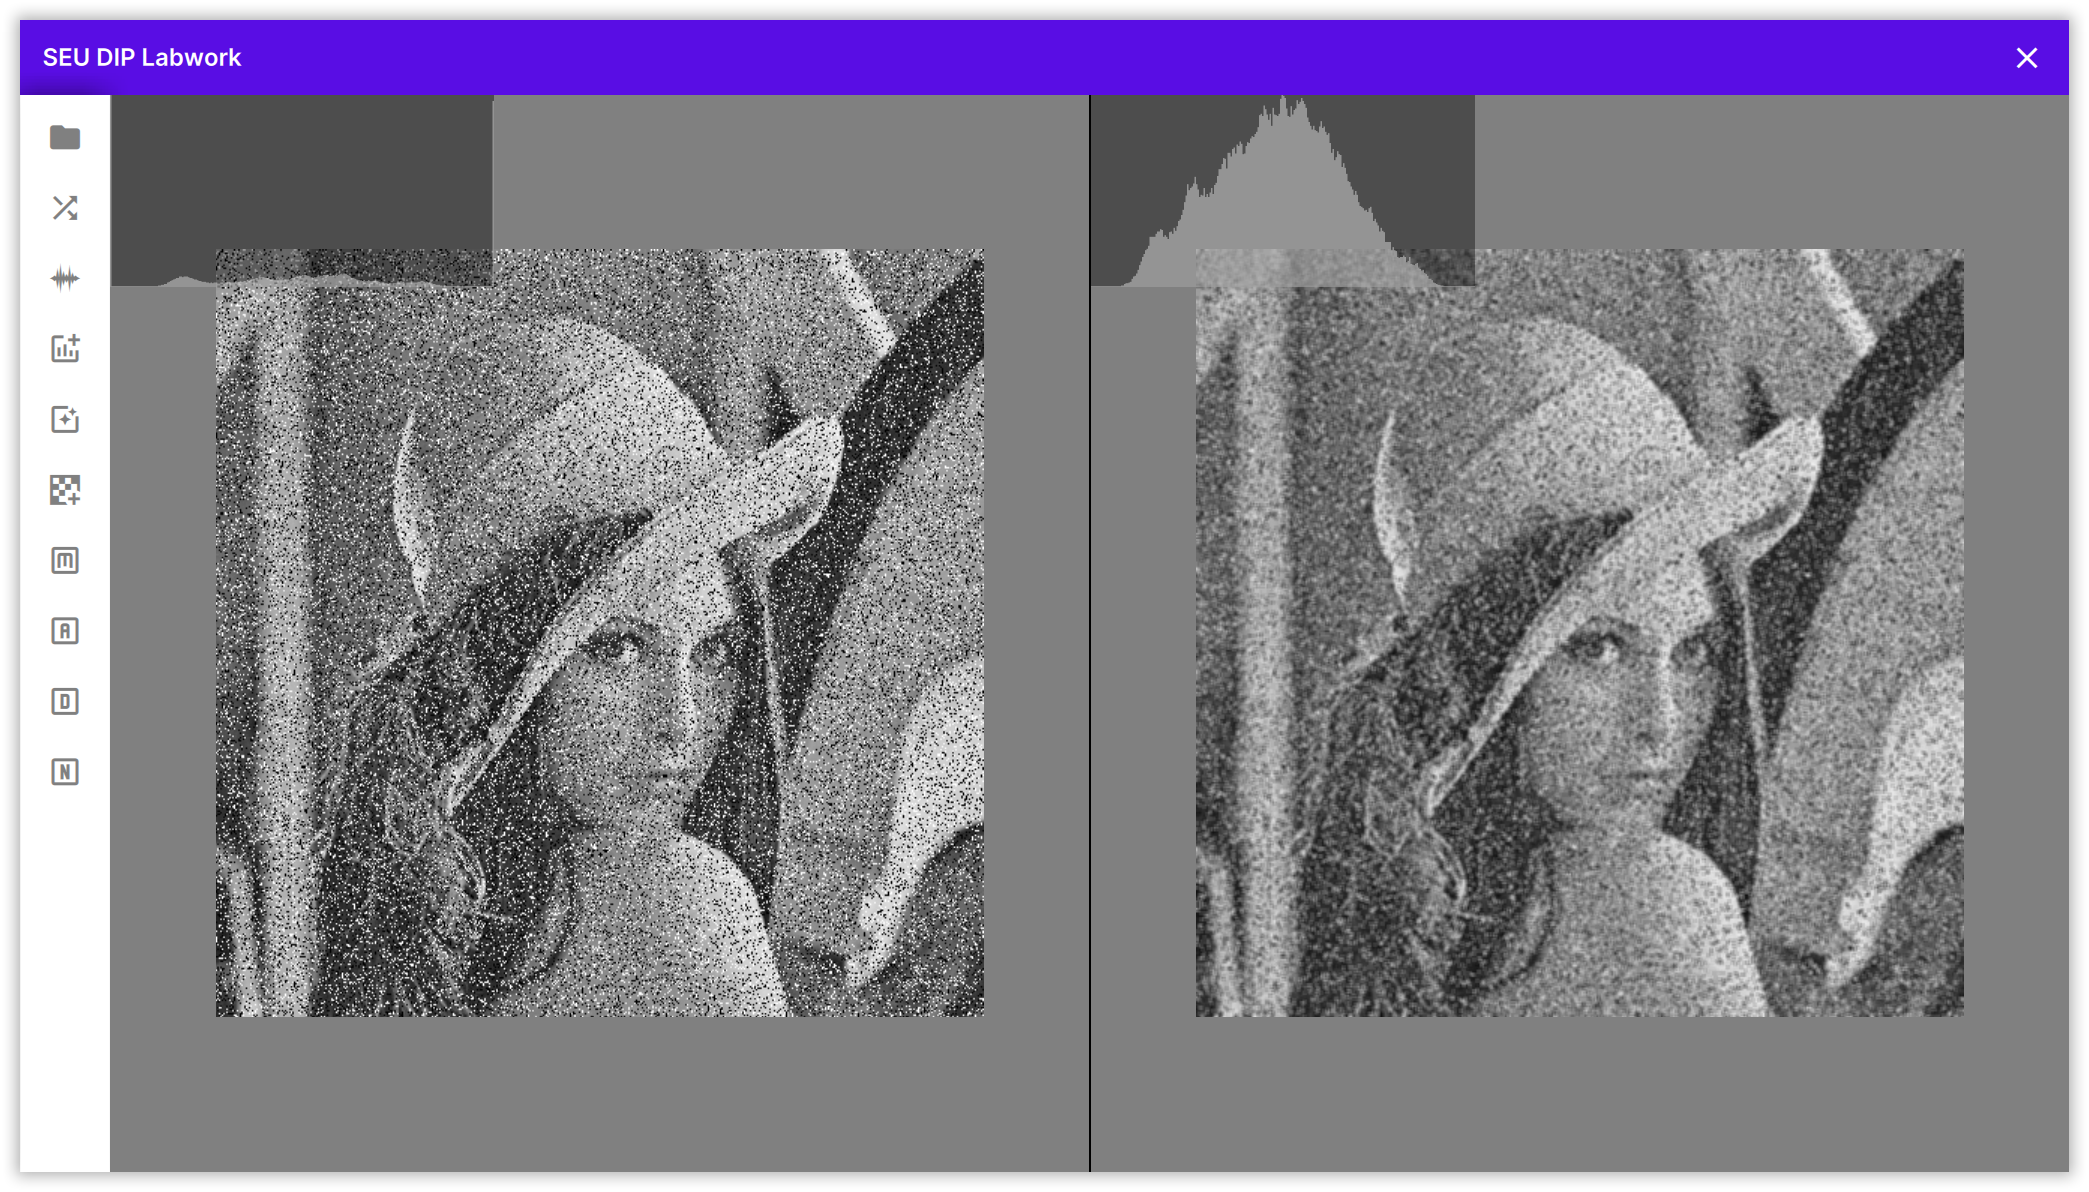
\includegraphics[width=\textwidth]{img/saltpepper/lena-avg.png}
    \caption{左侧为添加椒盐噪声之后的Lena图像,右侧是均值处理后的图像}
\end{figure}

\begin{figure}[H]
    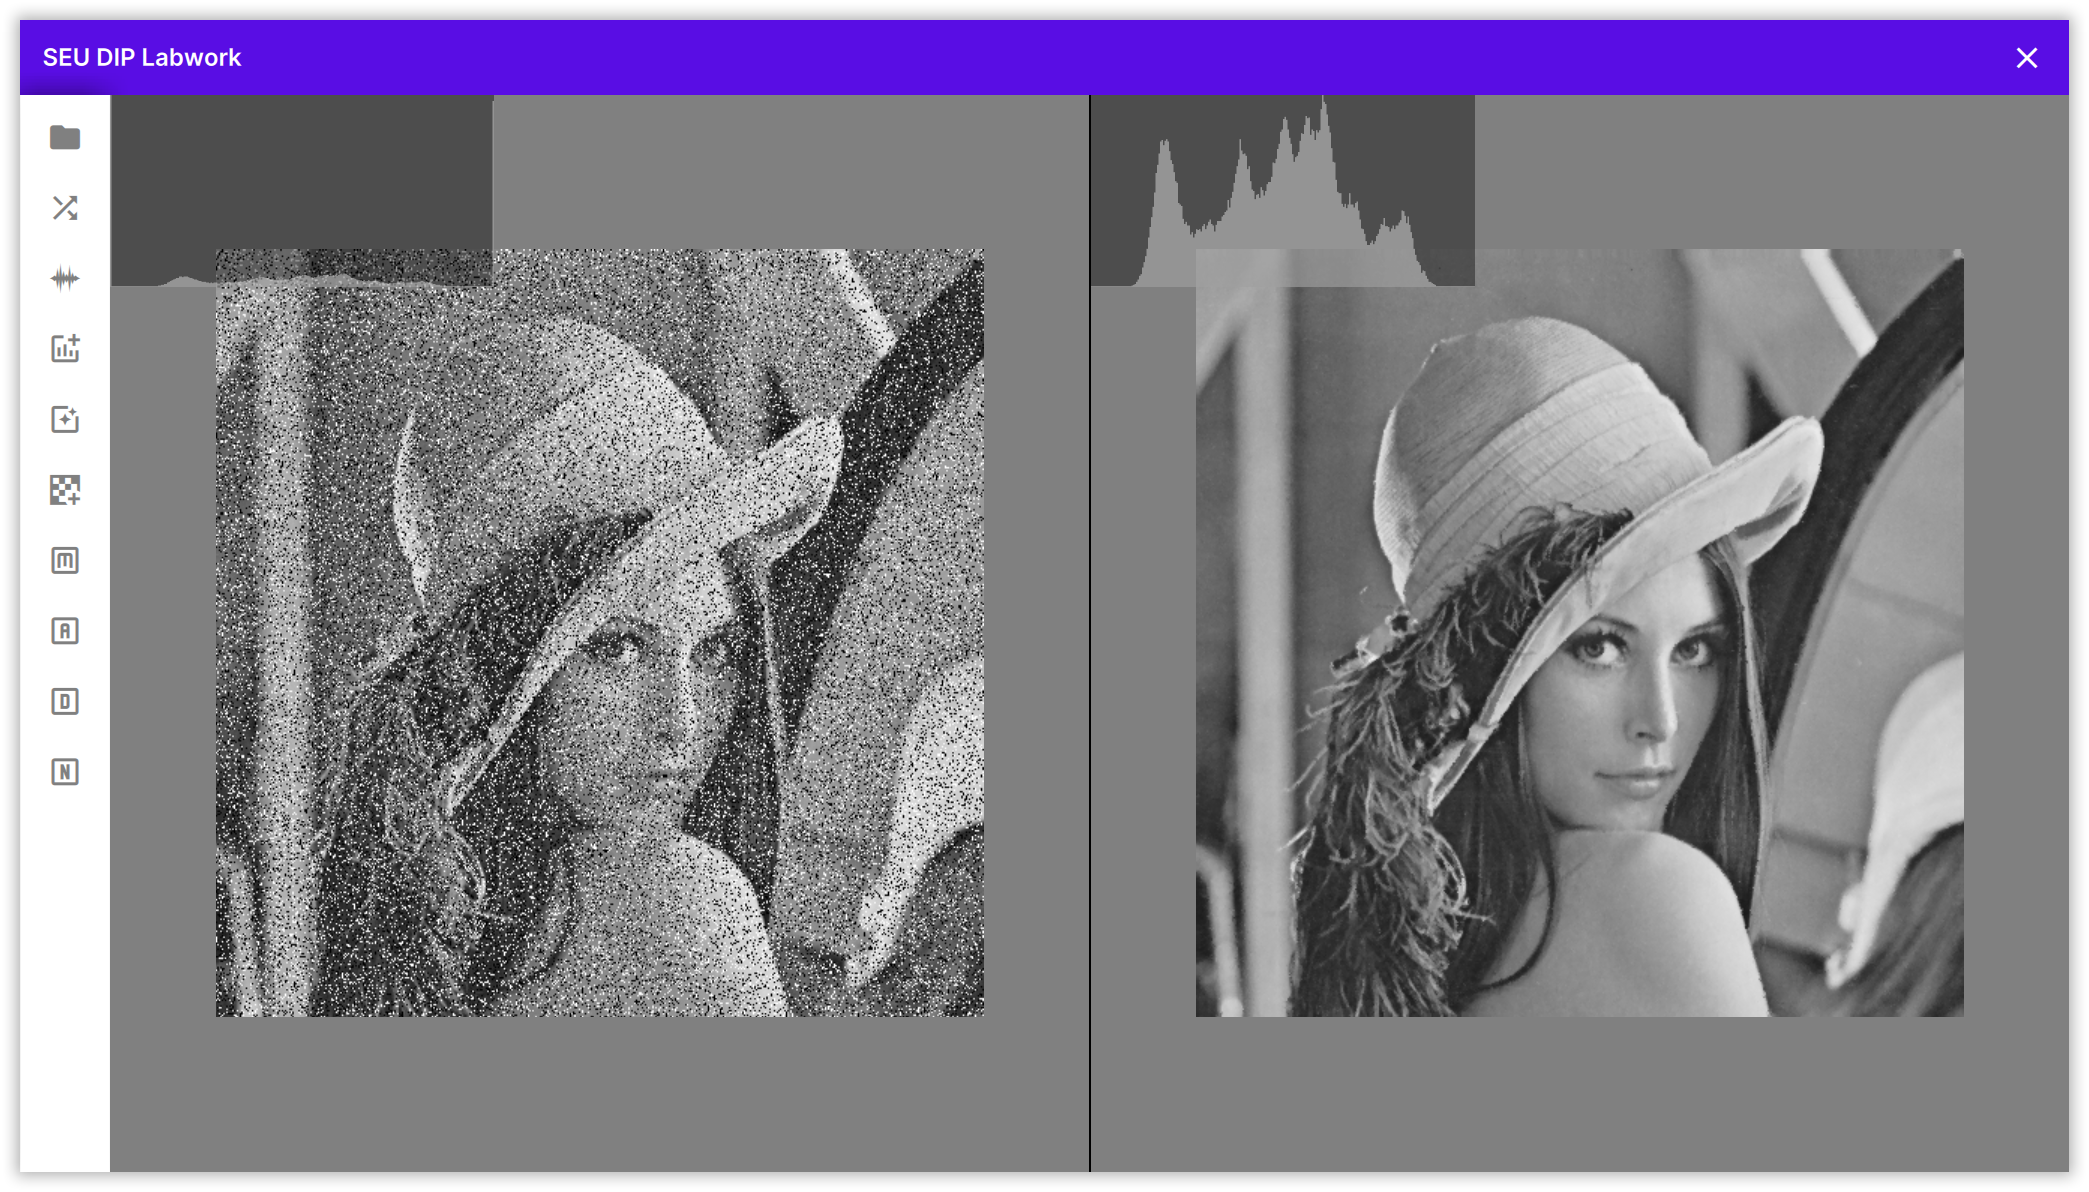
\includegraphics[width=\textwidth]{img/saltpepper/lena-adaptive.png}
    \caption{左侧为添加椒盐噪声之后的Lena图像,右侧是自适应中值处理后的图像}
\end{figure}

\begin{figure}[H]
    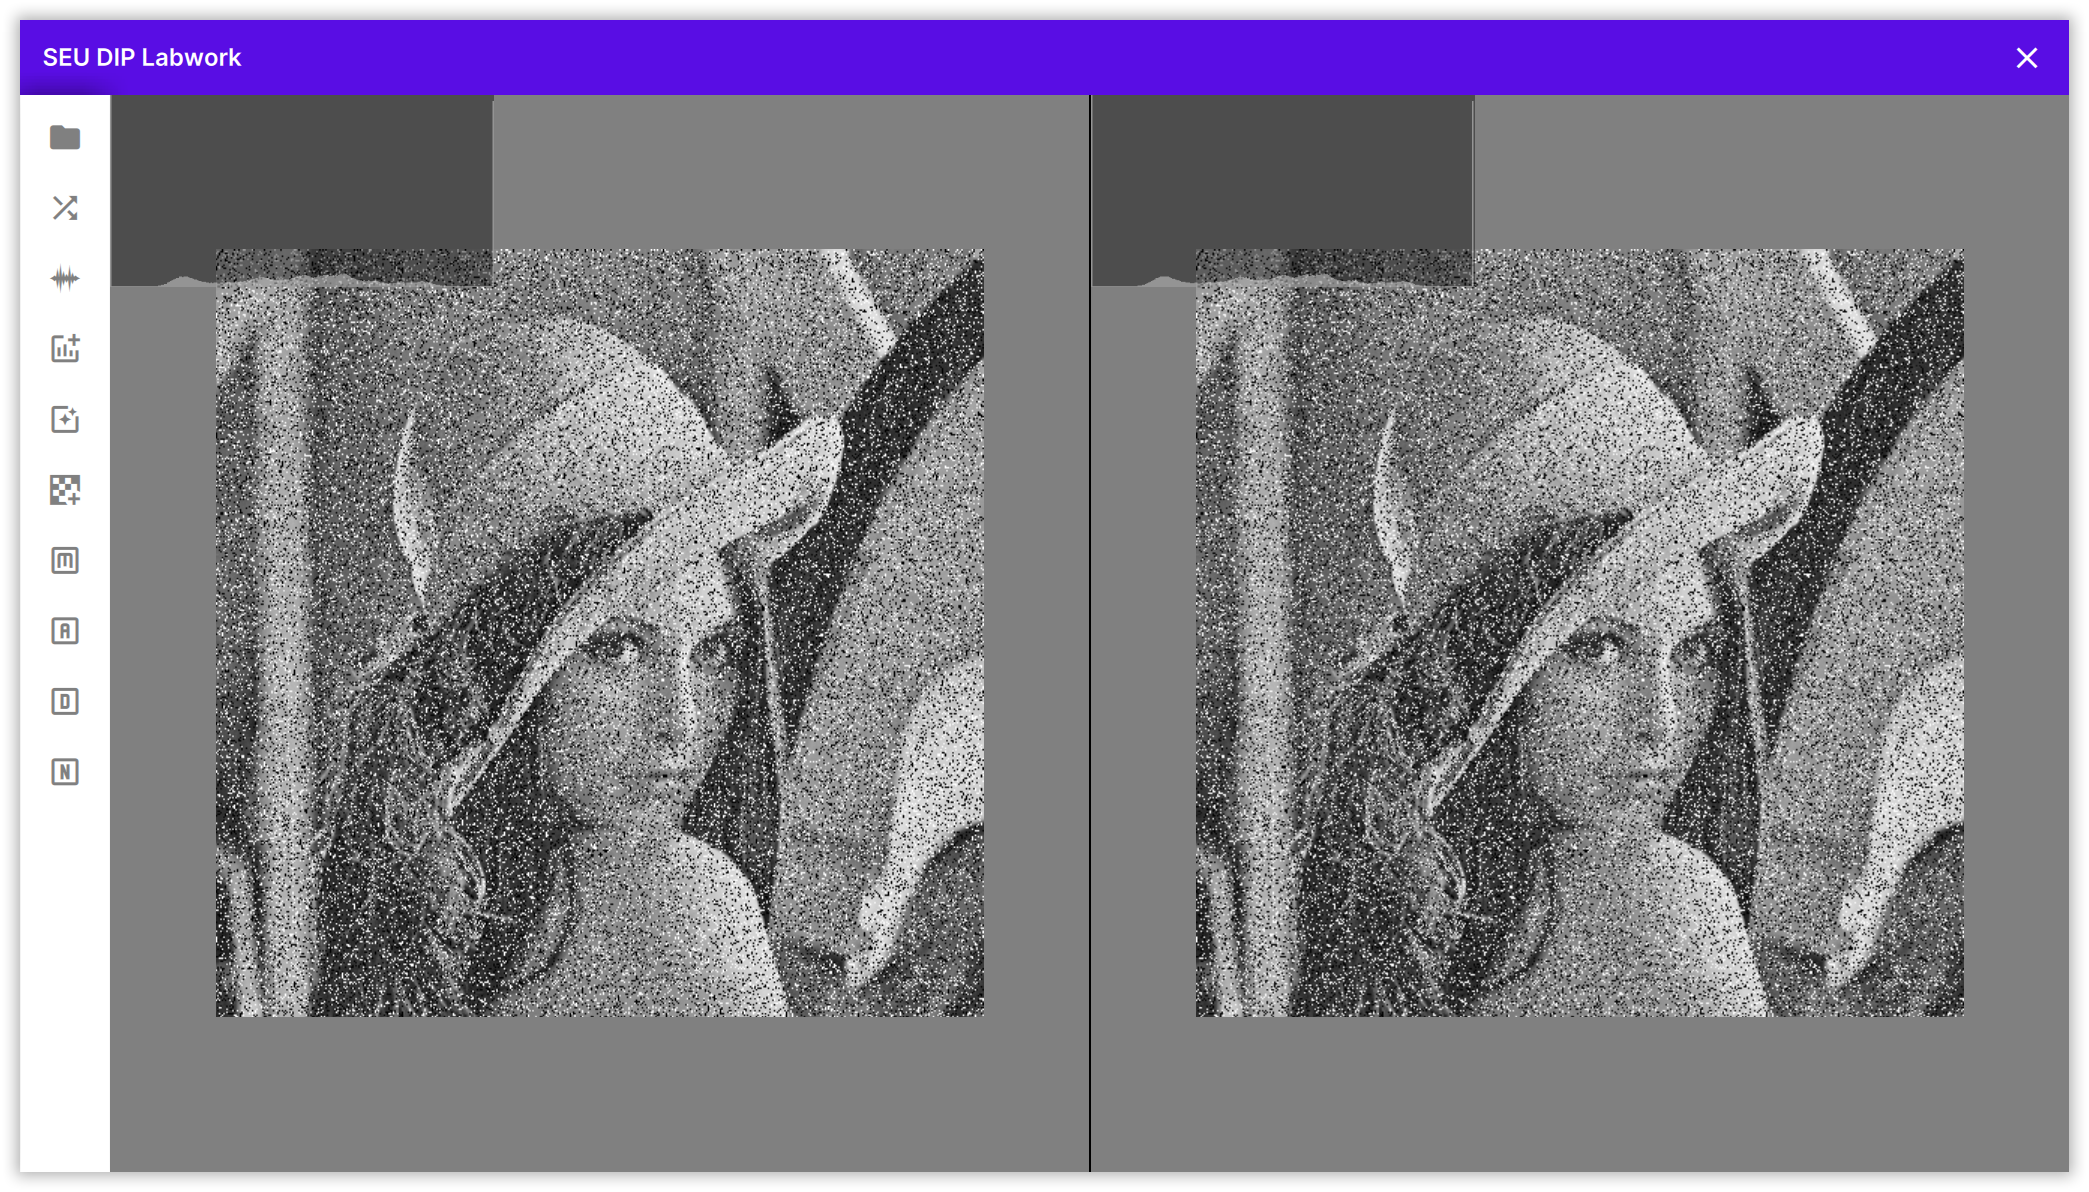
\includegraphics[width=\textwidth]{img/saltpepper/lena-nonlocal.png}
    \caption{左侧为添加椒盐噪声之后的Lena图像,右侧是Non-Local Means处理后的图像}
\end{figure}

可以看到,均值处理与Non-Local Means对于椒盐噪声的去除效果并不是很理想,而中值处理以及自适应中值处理有效的去除了椒盐噪声。其中,自适应中值处理较好的保留了图像的细节部分。

\end{document}
